%! TEX program = xelatex
% Paquetes:
\documentclass[letterpaper, 12pt]{article}
\usepackage[spanish]{babel} %%Paquete español para mac
\usepackage{graphicx} %% Para incluir figuras
\usepackage{xcolor}
\usepackage{ifpdf}
\DeclareGraphicsExtensions{.pdf}
\usepackage[margin=1in]{geometry}
\setcounter{totalnumber}{5}
\renewcommand{\textfraction}{0.1}
\usepackage[cmex10]{amsmath}
\usepackage{amssymb}
\usepackage{float}
\usepackage{cite}
\bibliographystyle{unsrt}
%\decimalpoint
\usepackage{url}
\usepackage{hyperref}
\hypersetup{colorlinks=false,bookmarksopen=true,linkbordercolor={1 1 1}}
%\usepackage{epstopdf}
\usepackage{mathtools}
\usepackage{chngcntr}
\usepackage{enumitem}
\providecommand{\e}[1]{\ensuremath{\times 10^{#1}}}
\usepackage[parfill]{parskip} % Líneas en lugar de indentación
\usepackage{fancyhdr}
\usepackage{booktabs}
\usepackage{cleveref}
\usepackage{verbatimbox}
\crefformat{footnote}{#2\footnotemark[#1]#3}

\usepackage[squaren]{SIunits} %esto me da nombres de unidades y prefijos
\usepackage{sistyle}% Esto es adecuado para escribir unidades.

\newcommand{\alumno}{Agustín Campeny}
\lhead{\nouppercase{\leftmark}}
\rhead{Tarea 4 - \alumno}
\pagestyle{fancy}
%\usepackage{scrextend}
\numberwithin{equation}{section}

\setlength{\tabcolsep}{6pt} % General space between cols (6pt standard)
\renewcommand{\arraystretch}{0.8} % General space between rows (1 standard)
\begin{document}
\thispagestyle{empty}
%%%%%%%%%%%%%%%%%%%%%%%%%%
%%%%%%%%% ENCABEZADO %%%%%%%%%
%%%%%%%%%%%%%%%%%%%%%%%%%%
\vspace*{-1cm}
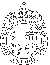
\includegraphics[width=2cm]{logo.pdf}
\vspace*{-2.2cm}

\hspace*{2cm}
 \begin{tabular}{l}
  {\ \textsc{\raggedright \footnotesize Pontificia Universidad Católica de Chile}}\\
  {\ \textsc{\raggedright \footnotesize Escuela de Ingeniería}}\\
  {\ \textsc{\raggedright \footnotesize Departamento de Ingeniería Eléctrica}}\\
  {\ \textsc{\raggedright \footnotesize IEE2753 - Diseño de Circuitos Integrados Digitales}}\\
  {\  }\\
 \end{tabular}
 \hfill
\vspace*{-0.2cm}
\begin{center}
  {\Large\bf Tarea 1}\\
\vspace*{2mm}
{\today}\\
\vspace*{2mm}
{\footnotesize \alumno}\\
\vspace*{6mm}
\end{center}
\hrule\vspace*{2pt}\hrule
%%%%%%%%%%%%%%%%%%%%%%%%%%
%%%%%%%%% ENCABEZADO %%%%%
%%%%%%%%%%%%%%%%%%%%%%%%%%

\section{Introducción}

En este reporte se presentan los resultados de los módulos \emph{RTL} implementados en el lenguaje \emph{verilog}, presentándose una breve introducción sobre la implementación, y las formas de onda resultantes de la simulación de los testbench respectivos.

Se utiliza el software \emph{Icarus Verilog} para la compilación y simulación de los testbench, y \emph{GTKWave} para la visualización de las formas de onda resultantes.

\section{Módulos RTL}

\subsection{Left Barrel Shifter}

Este módulo realiza la operación shift left de manera completamente combinacional. La implementación se encuentra basada en un documento por Matthew Rudolf Pillmeier\footnote{Barrel shifter design, optimization, and analysis, 2001}. Se implementa un módulo de largo variable definido por el parámetro \texttt{N}. A continuación se presentan formas de onda para varias entradas.

\begin{figure}[H]
  \centering
  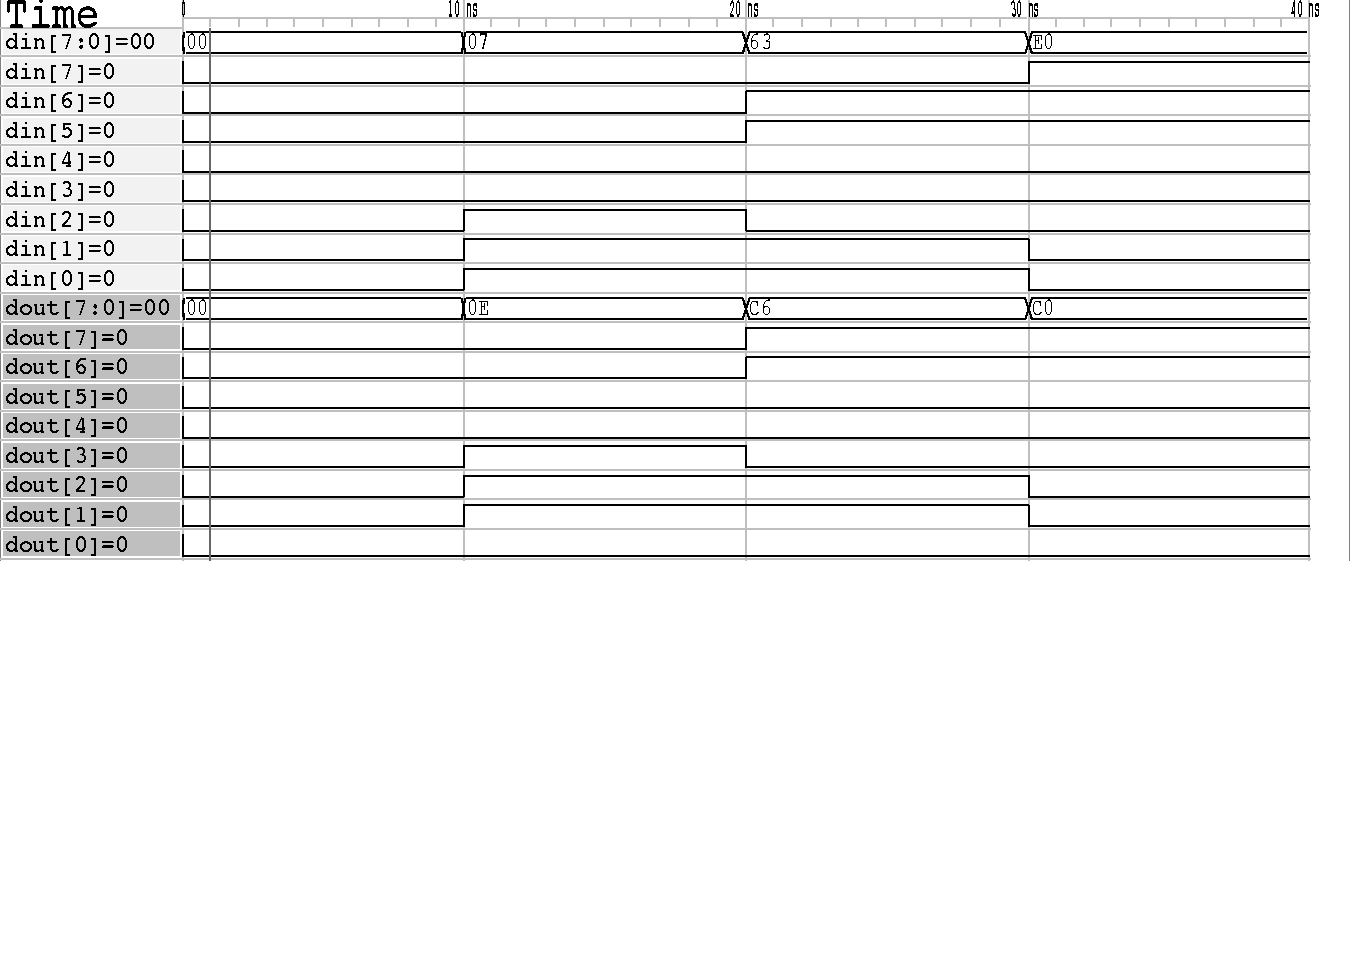
\includegraphics[width=0.9\textwidth]{../testbench/lbshifter/waves_lbshifter.pdf}
  \caption{Entrada y salida para diversos valores de largo 8 bits}
\end{figure}

\subsection{Addressable shift register}

Este módulo consiste en un shift register de 8 registros de largo variable. Se realiza un shift de los contenidos de cada registro en cada ciclo de reloj, y la salida corresponde a los contenidos del registro señalado por la dirección en la entrada \texttt{addr}. Este módulo fue basado en la descripción provista por Xilinx.\footnote{\url{https://www.manualslib.com/manual/195956/Xilinx-System-Generator-V2-1.html?page=26}}

La implementación se realizó mediante un arreglo de 8 registros de largo definido por el parámetro N. A continuación se presentan las formas de onda para distintas entradas y valores de dirección de salida.

\begin{figure}[H]
  \centering
  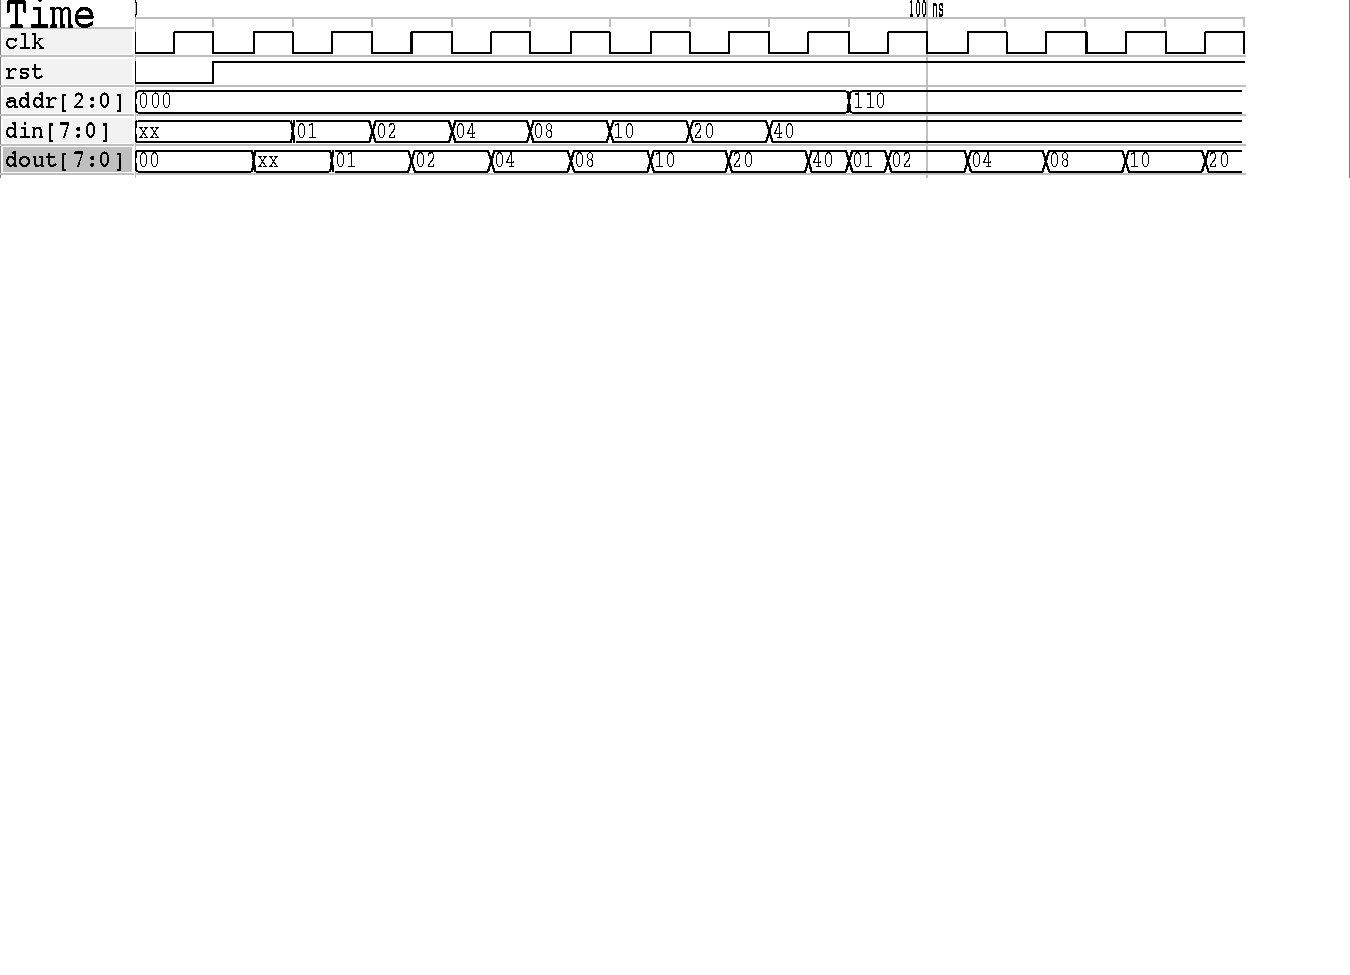
\includegraphics[width=0.9\textwidth]{../testbench/asr8/waves_asr8.pdf}
  \caption{Valores de salida correspondientes a la dirección en \texttt{addr}}
\end{figure}

\subsection{Linear-feedback shift register}

Se implementa un LFSR de tipo \emph{Fibonacci}, en el que el bit realimentado corresponde al XOR entre los bits de varias posiciones (denominadas ``taps'') dentro del registro.

La elección de los taps en este módulo fueron tal que el polinomio de realimentación fuese primitivo, con tal de asegurar un periodo máximo de \(2^n-1\), con \(n\) el largo en bits.\footnote{\url{https://en.wikipedia.org/wiki/Linear-feedback_shift_register}}. Se utilizó una tabla de polinomios publicada por E.J. Watson\footnote{Primitive Polynomials (mod 2)}, y se seleccionó el siguiente polinomio:

\begin{equation}
  x^{16}+x^{5}+x^{3}+x^{2}+1
\end{equation}

Al ser un LFSR de largo 16 bits, el periodo máximo es de 65535 valores diferentes antes de que se repita la secuencia. A continuación se presentan las formas de onda que prueban que esto se cumple.

\begin{figure}[H]
  \centering
  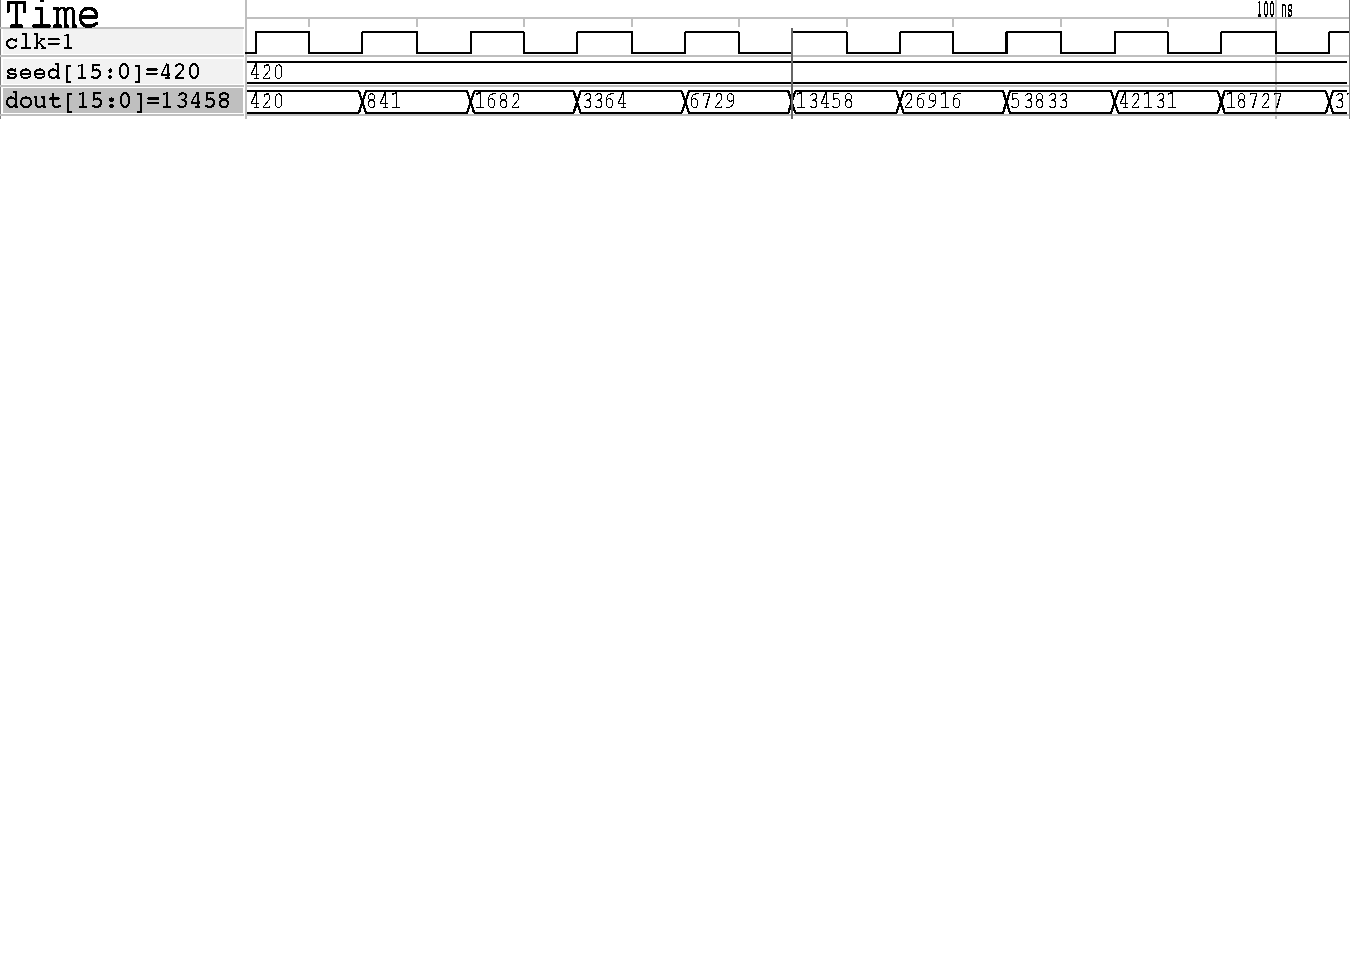
\includegraphics[width=0.9\textwidth]{../testbench/lfsr16/wave_lfsr_init.pdf}
  \caption{Seed inicial y primeros valores}
\end{figure}

\begin{figure}[H]
  \centering
  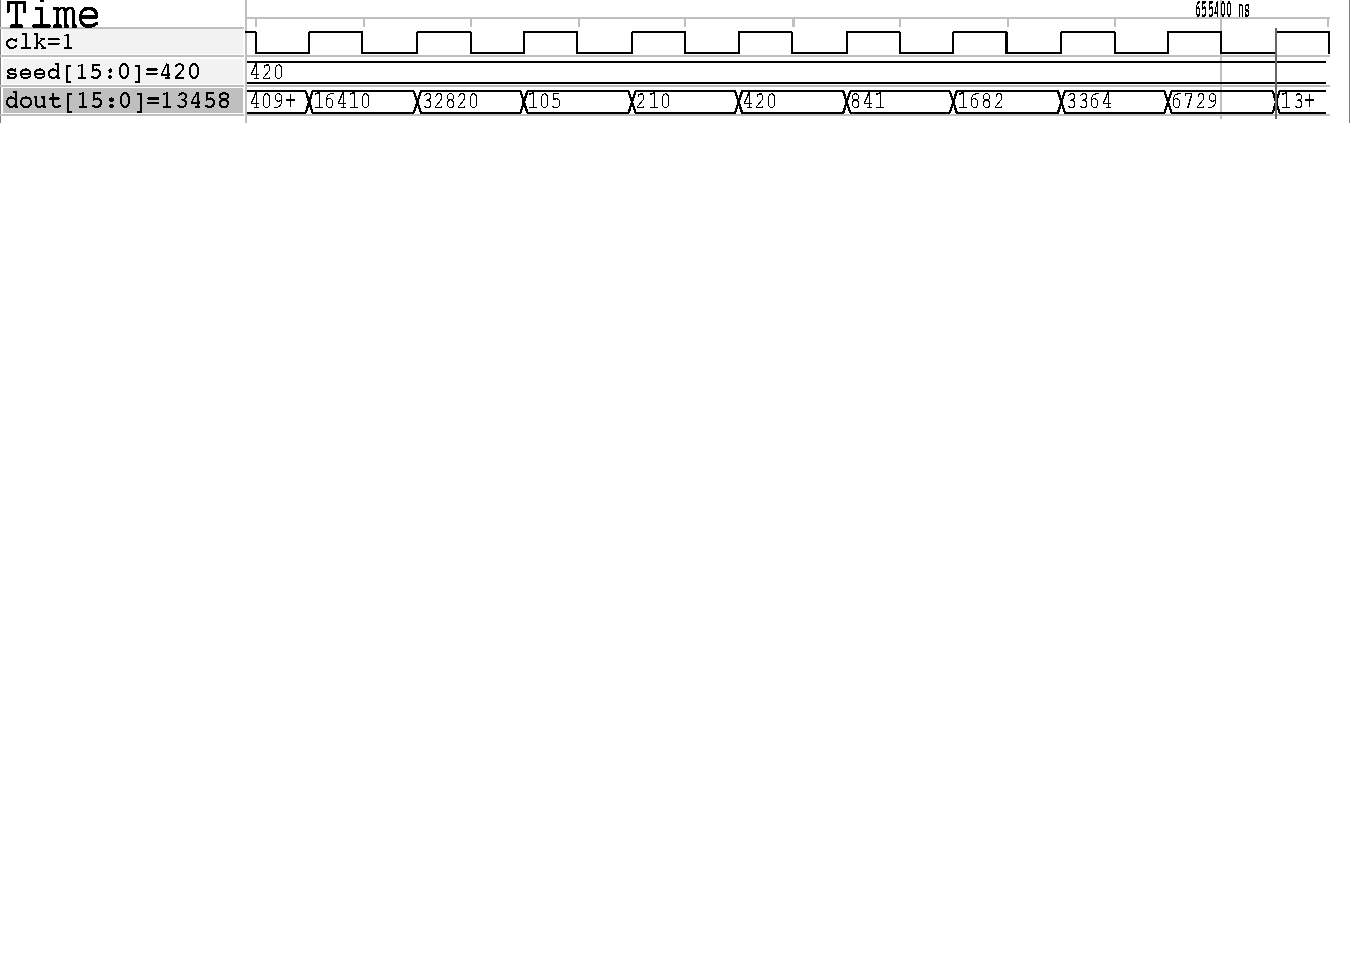
\includegraphics[width=0.9\textwidth]{../testbench/lfsr16/wave_lfsr_end.pdf}
  \caption{Reinicio del ciclo luego de 65535 ciclos}
\end{figure}

\subsection{Multiplier accumulator}

Este módulo multiplica los valores en sus entradas, y guarda el valor de la operación en un acumulador, el que corresponde a la salida de este\footnote{\url{https://en.wikipedia.org/wiki/Multiply–accumulate_operation}}. En los ciclos siguientes el valor del acumulador corresponde al valor anterior sumado al resultado de la multiplicación en dicho ciclo. Cada 8 ciclos se reinicia el valor del acumulador.

A continuación se presentan las formas de onda en donde se aprecia el valor del acunulador, y su reinicio en el ciclo 8.

\begin{figure}[H]
  \centering
  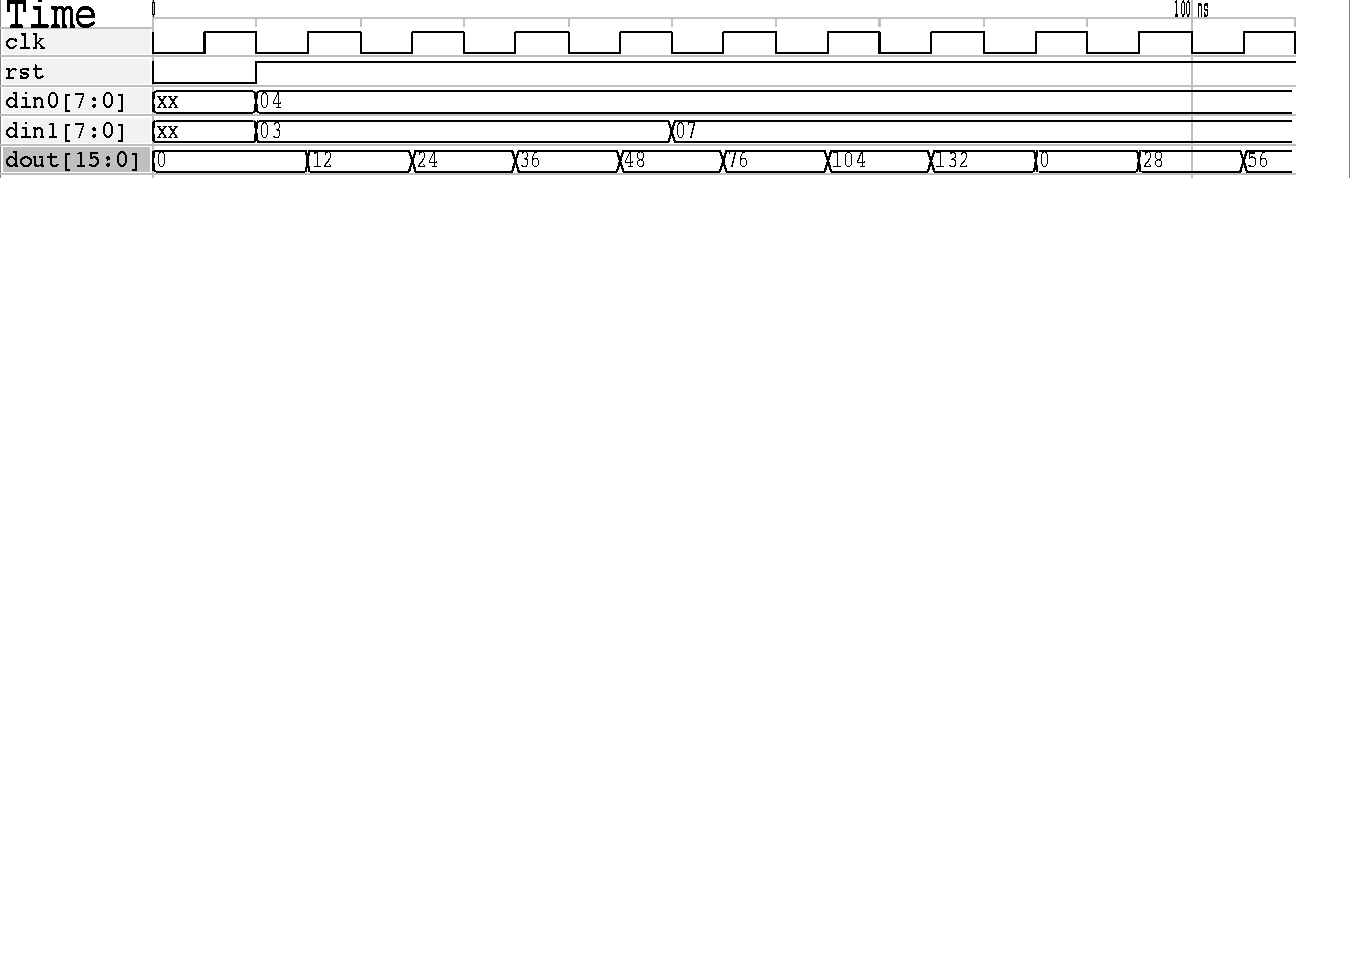
\includegraphics[width=0.9\textwidth]{../testbench/mac8/waves_mac8.pdf}
  \caption{Salida del módulo con respecto a las entradas y el número de ciclos}
\end{figure}






\end{document}
